\documentclass{alex_hü}

\name{Alexander Helbok}
\course{PS Physik}
\hwnumber{10}


\begin{document}
\renewcommand{\labelenumi}{\alph{enumi})}


\begin{mybox}{Stern–Gerlach Experiment}
	\centering \( v_x = 250 \unit{\v};\quad L_1 = 3.5 \unit{cm};\quad L_2 = 1 \unit{m};\quad B'_z = 1 \unit{T/cm} \)
	\tcblower
	\begin{enumerate}
		\item Silver Atoms are electrically neutral and therefore don't experience the lorentz force. Electrons however have spin, which cancels out for paired electrons. If the atoms has an unpaired (valence)electron in its outer shell, it creates a magnetic moment and therefore the atom interacts with magnetic fields. 
	\tcbline
		\item \( \Delta t_1 = \tfrac{L_1}{v_x};\quad \Delta t_2 = \tfrac{L_2}{v_x};\quad a_z = \tfrac{F_z}{m_{\text{Ag}}} = \tfrac{\mu_{\text{B}} B'_z}{m};\quad v_z = a_z\Delta t_2 \)
		\begin{flalign*}
			d &= v_z\Delta t_2 = \tfrac{L_1L_2\mu_{\text{B}} B'_z}{m_{\text{Ag}}v_x^2} = \dl{2.88 \times 10^{-3} \unit{m}} &&
		\end{flalign*}
	\tcbline
		\item Since the first magnet has already separated the atoms by spin, the second one should only deflect then even more, without splitting the atoms. We should therefore see a single dot on the detector.
	\tcbline
		\item The beam will be separated again in the y-Direction
	\end{enumerate}
\end{mybox}

%\begin{mybox}{Energieschema und Ubergänge in Rubidium}
%	\centering \(  \)
%	\tcblower
%	\begin{enumerate}
%		\item 
%	\tcbline
%		\item \(  \)
%%		\begin{flalign*}
%	%		
%%		\end{flalign*}
%	\tcbline
%		\item \(  \)
%%		\begin{flalign*}
%		%			
%%		\end{flalign*}
%	\tcbline
%		\item \(  \)
%%		\begin{flalign*}
%	%			
%%		\end{flalign*}
%	\end{enumerate}
%\end{mybox}

\begin{mybox}{Übersicht: Energieniveaus im Wasserstoffatom}
	\begin{minipage}{\textwidth}
		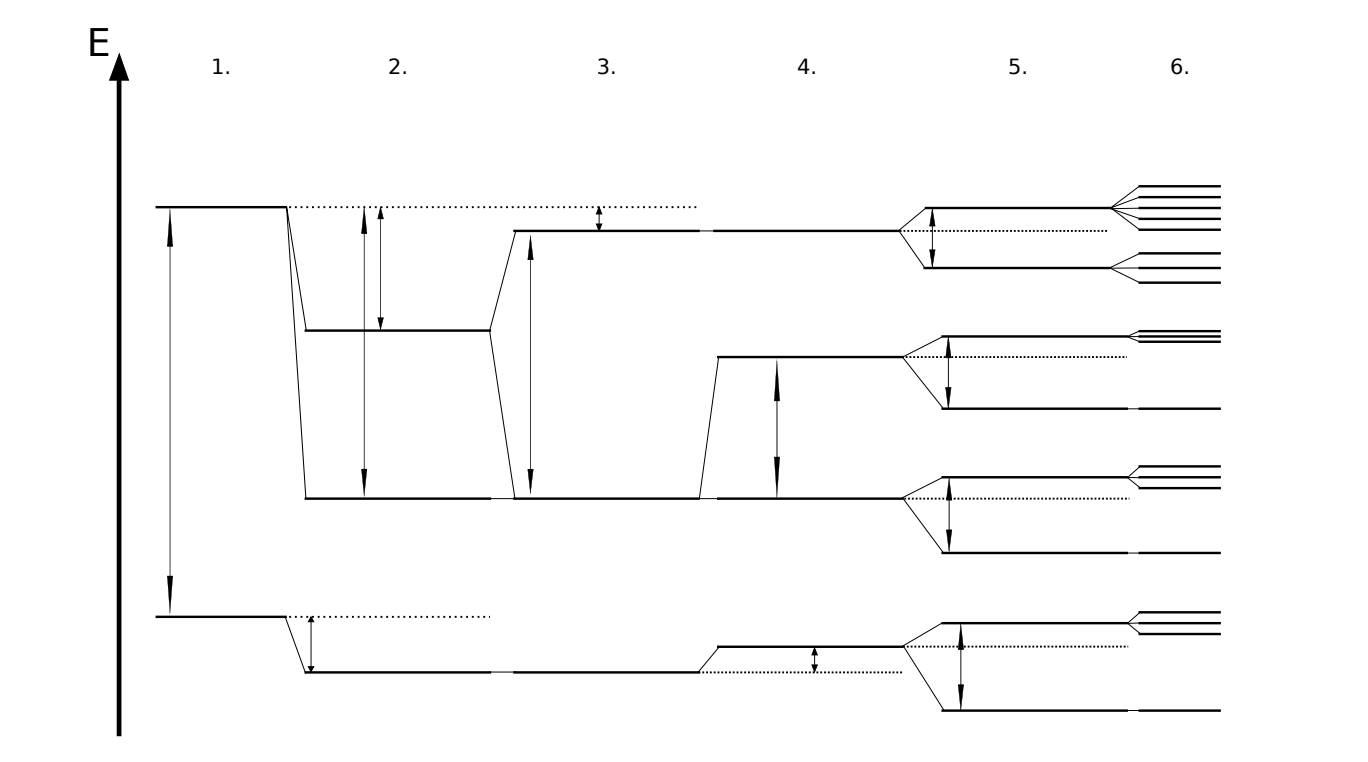
\includegraphics[scale=0.43]{energy}
	\end{minipage}
\end{mybox}


\end{document}